Variance reduction is a procedure used to increase the precision of the estimates that can be obtained for a given simulation, in order to make a simulation statistically efficient and obtain a greater precision and smaller confidence intervals for the output random variable of interest, variance reduction techniques can be used.The aim of this exercise is using some methods such as Antithetic variables, Control variates, Stratified sampling and importance sampling for variance reduction.
\subsection{The crude Monte Carlo estimator}
We want to estimate $\int_0^1 e^{x}dx$ by using crude Monte Carlo estimator based on 100 samples and present the result as the point estimator and a confidence interval.\\
This integral can be interpreted as
\begin{equation}
    E(e^U)=\int_0^1 e^{x}dx=\theta,        U\in U(0,1)
\end{equation}
TO estimate the integral,we sample of the random variable $e^U$ $(x_{i}=e^U_{i}$ and we take the average,\\
\begin{equation}
    \overline{X}=\frac{\Sigma^{i=1}_{n}X_i}{n}
\end{equation}
\subsection{Antithetic variables}
As mentioned before, doing simulation for estimating parameter $\theta=\overline{X}$ is more efficient if $Var(X)$ is reduced. Let identically distributed random variables $X_1$ and $X_2$ is generated then
\begin{equation}
    Var(\frac{X_1+X_2}{2})=\frac{1}{4}[var(X_1)+var(X_2)+2 Cov(X_1,X_2)]
\end{equation}
Variance is reduced if  $X_1$ and $X_2$ have $Cov(X_1,X_2)\leq 0$.
We want to estimate $\int_0^1 e^{x}dx$ by using Antithetic variables
\subsection{Stratified sampling}
Stratified random sampling is a method of sampling that involves the division of a population into smaller sub-groups known as strata. In  Stratified sampling members, the strata are formed based on shared attributes or characteristics such as income or educational attainment.\\
\\Table 5 shows the estimation of the integral for 3 different methods which is presented in sections 5.1, 5.2 and 5.3.

\subsection{Control variates}

In this part of exercise we used control variates to reduce the variance of the estimator in exercise 4 (Poisson arrivals).\\
Table 6 shows control variates which reduce the variance of the estimator in exercise 4.

\subsection{Simulation Result}

\begin{center}
    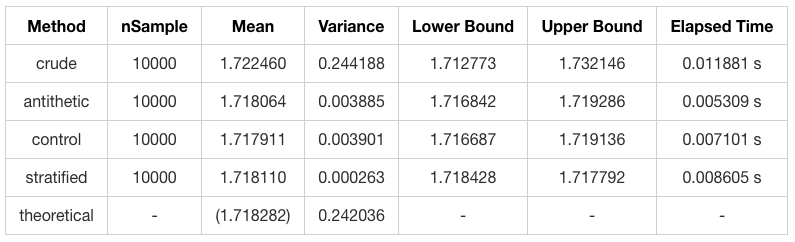
\includegraphics[scale=0.55]{Figures/figure5_1.png}\\
    \figuretitle{Table 5: Estimation of the integral by simulation. Present the point estimator and confidence interval.}
\end{center}\\

\begin{center}
    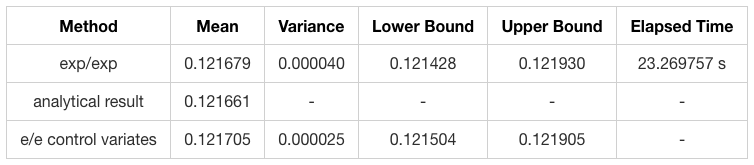
\includegraphics[scale=0.55]{Figures/figure5_2.png}\\
    \figuretitle{Table 6:Control Variates in Exercise 4.}
\end{center}\\